\documentclass{article}
\usepackage[margin=1in]{geometry}
\usepackage{amsmath,amsthm,amssymb}
\usepackage{bbm,enumerate,mathtools}
\usepackage{tikz,pgfplots}
\usepackage{chessboard}
\usepackage[hidelinks]{hyperref}
\usepackage{multicol} % Problem 35

\newenvironment{question}{\begin{trivlist}\item[\textbf{Question.}]}{\end{trivlist}}
\newenvironment{note}{\begin{trivlist}\item[\textbf{Note.}]}{\end{trivlist}}
\newenvironment{references}{\begin{trivlist}\item[\textbf{References.}]}{\end{trivlist}}
\newenvironment{related}{\begin{trivlist}\item[\textbf{Related.}]\end{trivlist}\begin{enumerate}}{\end{enumerate}}


\begin{document}
  Consider an $n$-coloring of a triangular grid such that no upright sub-triangle
  has the same coloring as any other (up to rotation).\\\vspace{0.5cm}

\begin{figure}[!h]
  \centering
  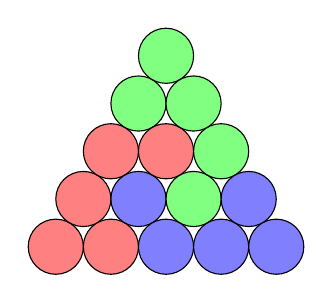
\begin{tikzpicture}[scale=0.7]
    \foreach \x/\y/\c in {
      0/0/red,  0/1/red,   0/2/red,   0/3/green, 0/4/green,
      1/0/red,  1/1/blue,  1/2/red,   1/3/green,
      2/0/blue, 2/1/green, 2/2/green,
      3/0/blue, 3/1/blue,
      4/0/blue} {
      \draw[fill=\c!50] (\x + 0.5 * \y, {\y * sqrt(3)/2}) circle (0.5cm);
    }
  \end{tikzpicture}\hspace{0.5cm}
  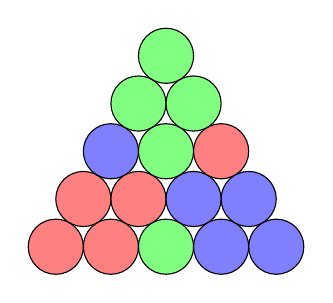
\begin{tikzpicture}[scale=0.7]
    \foreach \x/\y/\c in {
      0/0/red,   0/1/red,  0/2/blue,  0/3/green, 0/4/green,
      1/0/red,   1/1/red,  1/2/green, 1/3/green,
      2/0/green, 2/1/blue, 2/2/red,
      3/0/blue,  3/1/blue,
      4/0/blue} {
      \draw[fill=\c!50] (\x + 0.5 * \y, {\y * sqrt(3)/2}) circle (0.5cm);
    }
  \end{tikzpicture}\hspace{0.5cm}
  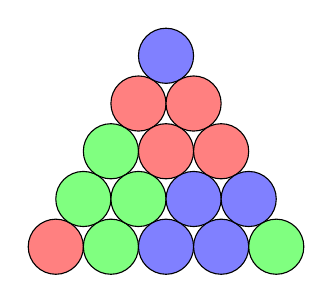
\begin{tikzpicture}[scale=0.7]
    \foreach \x/\y/\c in {
      0/0/red,  0/1/green,   0/2/green,   0/3/red, 0/4/blue,
      1/0/green,  1/1/green,  1/2/red,   1/3/red,
      2/0/blue, 2/1/blue, 2/2/red,
      3/0/blue, 3/1/blue,
      4/0/green} {
      \draw[fill=\c!50] (\x + 0.5 * \y, {\y * sqrt(3)/2}) circle (0.5cm);
    }
  \end{tikzpicture}\hspace{0.5cm}
  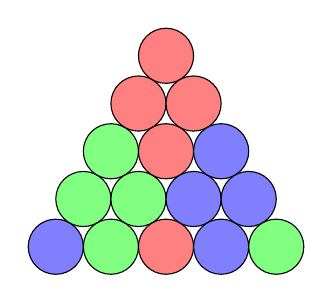
\begin{tikzpicture}[scale=0.7]
    \foreach \x/\y/\c in {
      0/0/blue,  0/1/green,   0/2/green,   0/3/red, 0/4/red,
      1/0/green,  1/1/green,  1/2/red,   1/3/red,
      2/0/red, 2/1/blue, 2/2/blue,
      3/0/blue, 3/1/blue,
      4/0/green} {
      \draw[fill=\c!50] (\x + 0.5 * \y, {\y * sqrt(3)/2}) circle (0.5cm);
    }
  \end{tikzpicture}

  \caption{
    Four examples of 3-colorings of the length 5 triangle.
    In all cases, 10 different colorings appear exactly once. In the first
    example, starting from the top:
    (1) GGG, (2) RRG, (3) RGG, (4) RRB, (5) RGB, (6) GGB, (7) RRR, (8) RBB,
    (9) GBB, and (10) BBB.
    (Incidentally, this is \textit{all} of the colorings, so $a(5) = 3$.)
  }
\end{figure}

\begin{question}
  Given $n$ colors, what is the biggest triangle that can be constructed?
  Call the side length of such a triangle $a(n)$.
\end{question}
\begin{related}
  \item What if inverted triangles are counted too?
  \item What if two triangles with the same coloring but different rotations are
    counted as different?
  \item How many patterns exist for a triangle of length $k$ with the minimum
    number of labels?
  \item What if diagonal equilateral triangles are also considered?
    (For example, take the second circle on every side as measured clockwise
    from each corner.)
  \item What if this is done on a square grid?
  \item What if this is done on hexagonal shapes?
  \item What if this is done on tetrahedra or cuboids?
  \item Consider the lexicographically earliest infinite case. Does every
    triangle eventually appear?
\end{related}
\begin{references}
  \item \url{https://math.stackexchange.com/a/2416790/121988}
  \item \url{https://math.stackexchange.com/a/2636168/121988}
\end{references}
\end{document}
